\graphicspath{{/Users/emiliendurif/Documents/prepa/sujets/TP_simulation/axenum/}}
\subsection{Introduction}
\subsubsection{Objectifs}

On souhaite améliorer les performances du système AxNum lorsqu'il est asservi en vitesse. Le cahier de charges de l'axe prototype impose un temps de réponse à $95\%$ inférieur à $0,5s$. Afin d'améliorer nos connaissances du système et tester rapidement différents réglages, une simulation va être développée. Des difficultés de modélisation inhérentes à ce type de système comme les effets de seuil provenant des frottements secs ou les effets de saturation provenant des limitations des composants seront observés.

\subsubsection{Système}

Nous étudierons l'axe numérique Didalab Figure \ref{Figure1}. Ce système permet le positionnement ou la régulation de vitesse d'un chariot motorisé par une machine à courant continu. Il pourrait servir à positionner la tête d'impression d'une imprimante 3D, la broche d'une machine-outil (avec un moteur plus puissant) ou encore la tête d'une imprimante grandes dimensions. Cet axe permet de faire des expériences dans un environnement de prototypage contrôlé et de valider des choix techniques avant de réaliser une machine plus complète. Idéalement cet axe doit être rapide et précis, des critères quantifiés étant disponibleS dans le cahier des charges de la machine que l'on souhaite réaliser.
Une alimentation 24V 2.9A est utilisée. Dans le boitier se trouvent une carte électronique à microcontrôleur pour les calculs et la correction ainsi qu'une carte électronique de puissance à transistors MOSFET. Cette carte est contrôlée par un logiciel sur PC.

\begin{figure}[!htb]
\begin{center}
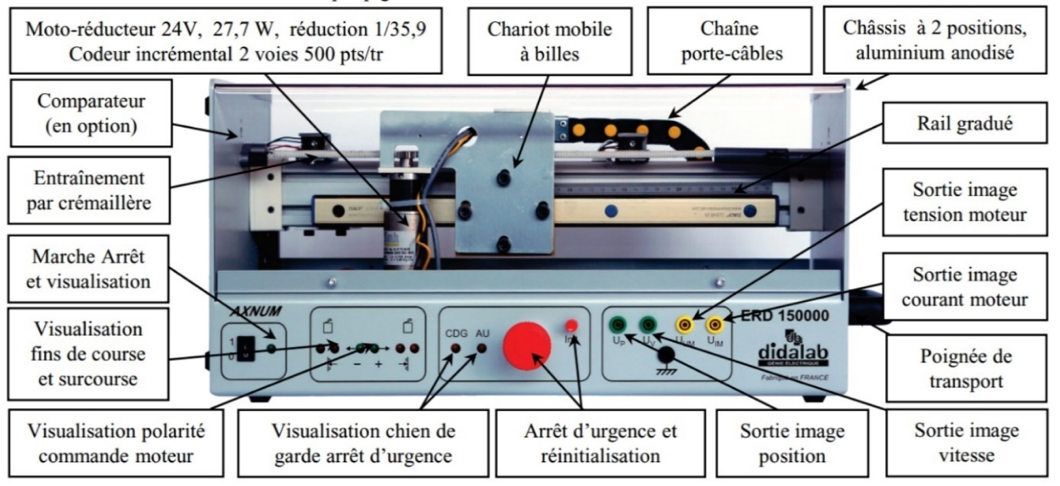
\includegraphics[width=1.0\textwidth]{images/figure1.png}
\caption{Présentation de l'axe numérique \label{Figure1}}
\end{center}
\end{figure}

\subsubsection{Présentation de Matlab Simulink}

Matlab est un langage de programmation dédié aux ingénieurs et aux scientifiques. Il dispose de nombreuses similarités avec Python : Il ne se compile pas et le typage est faible : par exemple il n'est pas nécessaire de déclarer le nom ou le type (booléen, entier, flottant, ...) des variables avant de les utiliser. L'interpréteur se charge de « deviner » les intentions en fonction du type de calcul. Matlab est un logiciel propriétaire. Il dispose d'un environnement de programmation intégré : éditeur de texte, interpréteur bibliothèques et éléments de visualisation sont dans un même package.
Matlab intègre aussi de nombreux outils dédiés aux problèmes scientifiques et d'ingénierie que l'on ne retrouve pas dans Python. Par exemple Simulink est un outil permettant de mettre en place des modèles par schéma blocs avec une interface graphique et un solveur intégré. Ainsi l'utilisateur dispose les blocs dans une fenêtre, les relie, définit les équations de leurs fonctions de transfert, les entrées et les sorties souhaitées. Ensuite il peut résoudre et nous permettre d'observer les résultats de la modélisation. Simulink est très largement utilisé dans l'industrie (aérospatiale, environnement, défense etc...). Par rapport à une résolution analytique l'ordinateur permet de traiter des systèmes plus complexes et éventuellement de s'affranchir des hypothèses linéarité/continuité/invariance indispensable dans une étude analytique. Simulink permet aussi de s'interfacer avec du matériel (carte de mesure, système physique) ou d'autre logiciel (Solidworks, meca3D).

\subsubsection{Déroulement du TP}

\begin{enumerate}
\item	Analyse de la chaine fonctionnelle.
\item Mise en place d'un modèle de connaissance avec schéma bloc, axe en boucle ouverte.
\item Prise en main de Simulink.
\item Modélisation de l'axe numérique en boucle ouverte et interface de courant.
\item Mise en place d'un modèle de connaissance avec schéma bloc, axe en boucle fermée.
\item Modélisation de l'axe numérique en boucle fermée de vitesse et interface de courant.
\item Modélisation de l'axe numérique en boucle fermée de position et interface de courant.
\item Modélisation de l'axe numérique en boucle fermée de position avec retour tachymétrique et interface de courant.
\end{enumerate}

\subsection{Analyse structurelle du système}
\subsubsection{Chaine fonctionnelle du système}

\question{Placer Codeur incrémental, Chariot, Alimentation $24V$, Pignon-crémaillère, Moteur, réducteur, carte électronique de puissance, carte électronique à microcontrôleur, logiciel PC, boutons, Leds. sur la chaine fonctionnelle ci-dessous}

\begin{center}
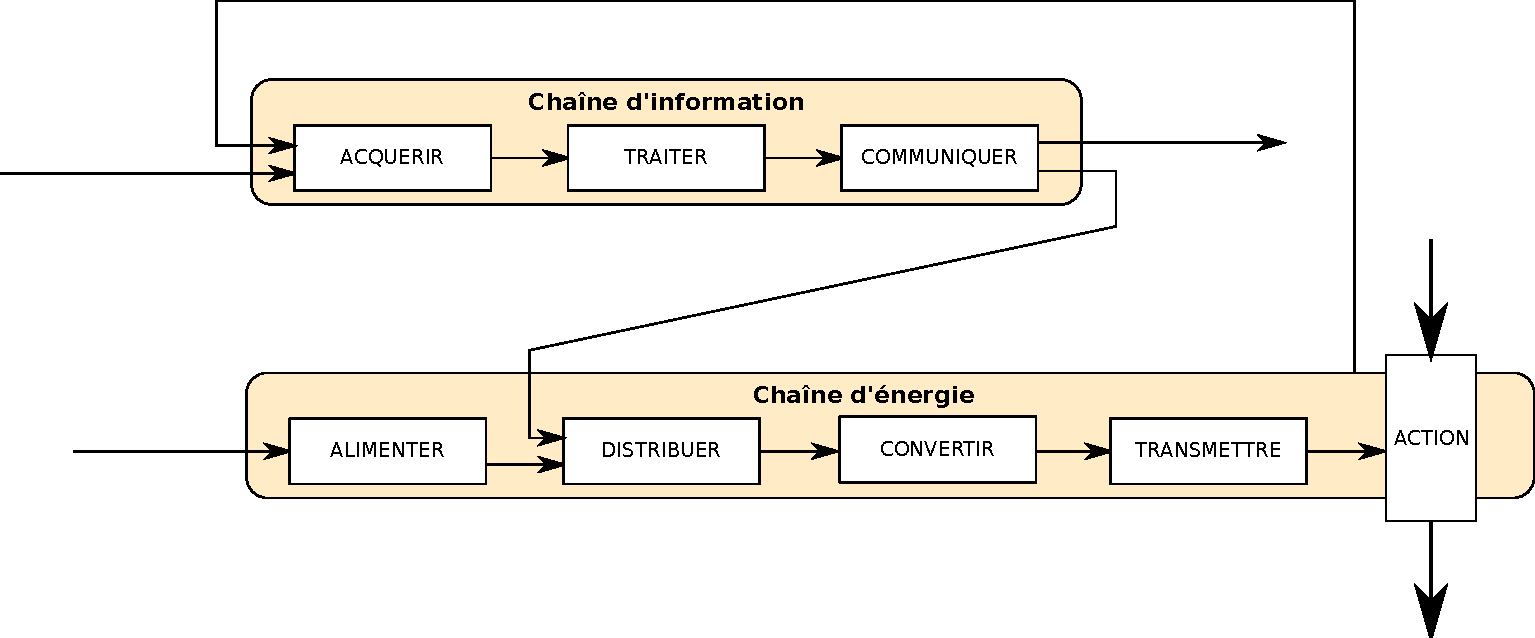
\includegraphics[width=1.0\textwidth]{images/chaine_fonctionnelle_vierge.pdf}
\end{center}

\subsubsection{Modélisation en boucle ouverte à l'aide d'un schéma bloc}

Ou souhaite étudier l'évolution temporelle de la vitesse du chariot (dans le cadre de la future étude en mode asservi). En boucle ouverte le logiciel permet de contrôler le courant d'alimentation. 

\question{Identifier l'entrée et la sortie du modèle recherché (indispensable pour identifier le contenu des blocs).}

On donne : 
\begin{itemize}
\item Documentation du motoréducteur et du pignon (annexe 1) :
\begin{itemize}
\item Constante de couple notée $K_i=4,32N\cdot cm\cdot A^{-1}$ ;
\item Moment d'inertie du moteur $J=0,043\cdot 10^{-4}kg\cdot cm^2$ (négligeable) ;
\item Inertie au niveau du réducteur négligeable et rendement égal à 1.
\item Rapport de réduction du réducteur $K_{red}=35,9$ ;
\end{itemize} 
\item Diamètre primitif d'un pignon : $D = m Z$ avec $m=0,8$ le module (ici en $mm$) et $Z=21$ le nombre de dents. 
\item Masse équivalente du chariot : $M_{eq}=120 Kg$ (masse chariot et inertie motoréducteur combinées).
\end{itemize}

\question{Placer les éléments suivants : Couple réducteur $C_r$, Force motrice $F$, Courant commande $I_m$, Couple moteur $C_m$, Accélération $M_x''$, et Vitesse $M_x'$. Les gains ou fonctions des blocs sont ensuite à spécifier. Une intégration et une équation du mouvement seront nécessaires. Une attention particulière sera portée aux unités.}

\ifthenelse{\boolean{corrige}}
			{\
\begin{center}
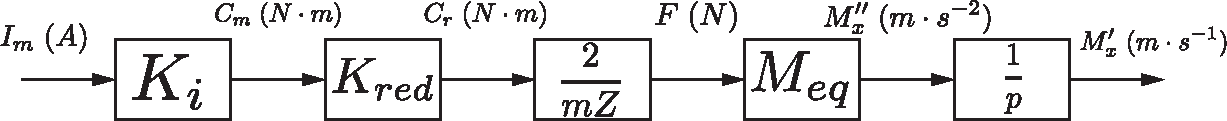
\includegraphics[width=1.0\textwidth]{images/BO_complet.pdf}
\end{center}					
			}
			{
\begin{center}
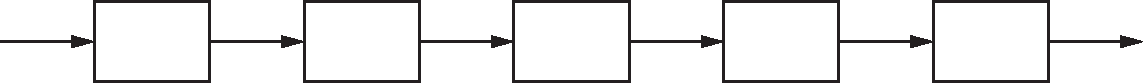
\includegraphics[width=1.0\textwidth]{images/BO_vide.pdf}
\end{center}		
			}
			
\subsection{Comparaison des performances en boucle ouverte : utilisation de Matlab Simulink}

\subsubsection{Prise en main de Matlab Simulink}

\begin{itemize}
\item Créer un répertoire SimAxnum à la racine de $U:\backslash Perso$. Lancer MATLAB (dernière version). Placer l'adresse du répertoire dans la barre d'adresse de Matlab. 
\item Tester le mode calculatrice en tapant un calcul dans la barre d'exécution en bas de l'écran. 
\item Faites click gauche dans la fenètre de gauche « New Script » pour créer un fichier de commandes Matlab dans le répertoire de travail. Ce fichier permettra de faire des calculs, des programmes et de définir des variables ce qui sera utile pour Simulink. Par exemple taper « A=3+pi » dans le script et l'exécuter (onglet lecture). La variable A apparait dans le « Workspace ». 
\begin{center}
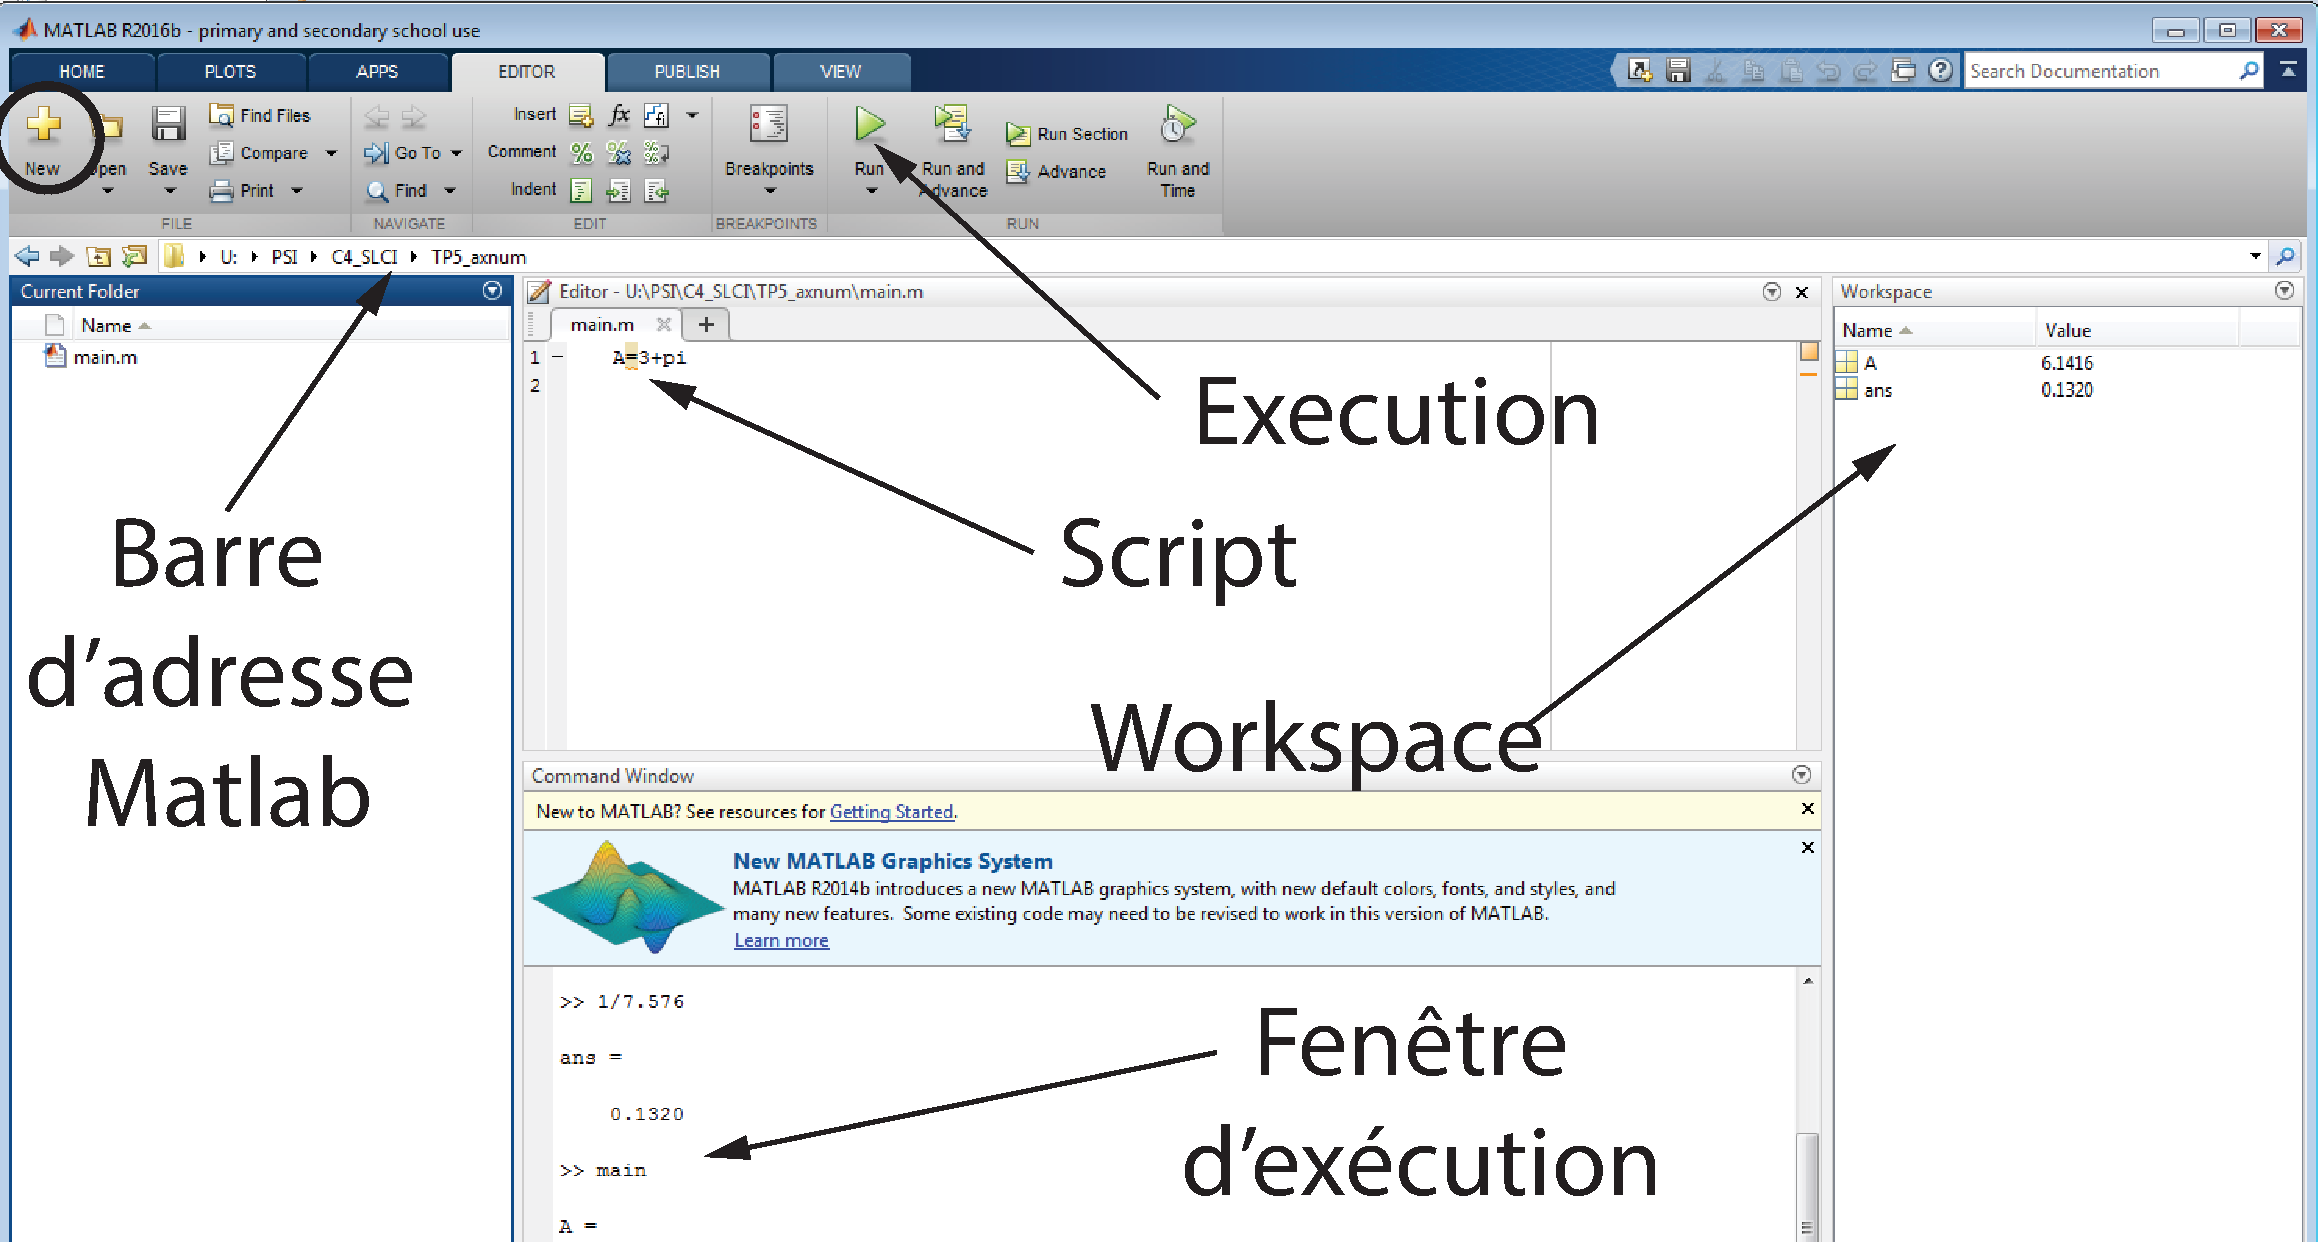
\includegraphics[width=0.8\textwidth]{images/matlab1.pdf}
\end{center}

\item Désormais presser le bouton Simulink dans l'onglet "Home" puis choisir un « Blank model » pour créer votre premier schéma bloc à simuler. 

\begin{center}
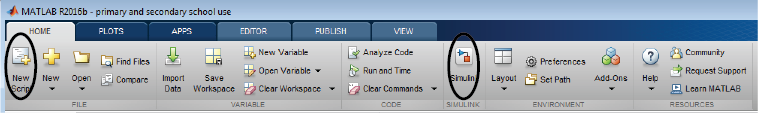
\includegraphics[width=0.8\textwidth]{images/matlab_simulink.png}
\end{center}

\item En pressant le bouton de couleur on peut choisir ses blocs (librairie Simulink). Dans les rubriques « commonly used block » (blocs courants) « source » (entrées) « sinks » (sorties) « continuous » (intégrale, dérivé, fonction de transfert) et « Math » (polynomes, trigonométrie, seuils) vous trouverez l'essentiel des blocs de base dont vous aurez besoin.

\begin{center}
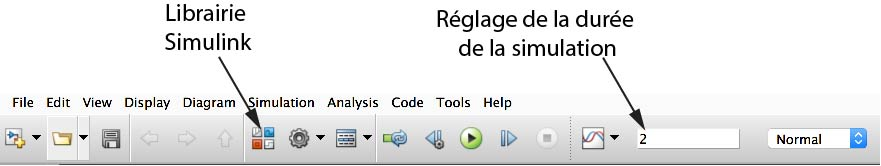
\includegraphics[width=0.8\textwidth]{images/matlab2.jpg}
\end{center}

\item Glisser un signal échelon « source » dans le nouveau modèle et paramétrez le à la valeur finale 3, ajoutez un bloc "transfert function" de manière à modéliser un premier ordre avec une constante de temps égale à 1. Ajouter un bloc Scope « sink » et un bloc "to workspace". Reliez-les et exécutez (bouton lecture). Ouvrir le scope et commenter le résultat. Observer dans le workspace les variables créées.

\begin{center}
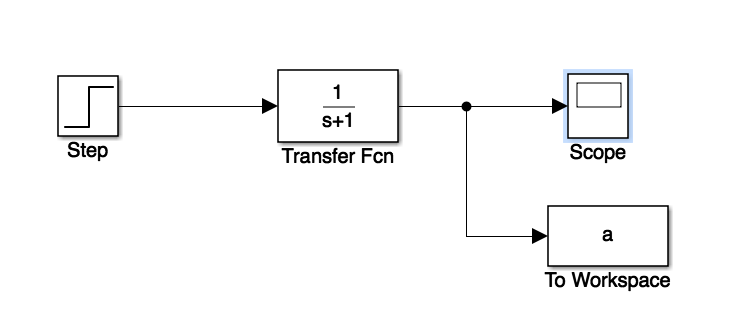
\includegraphics[width=0.6\textwidth]{images/simulink_1er_ordre.png}
\end{center}

\item Taper $a$, puis $a\cdot Time$ et $a.Data$ dans la fenêtre d'exécution.

\end{itemize}

\subsubsection{Simulation du schéma bloc en boucle ouverte}

Vous trouverez dans le dossier TP5 Transfert un dossier nommé "axnum$\_$eleves". Copier les fichiers qu'il contient dans le dossier créé dans votre dossier perso.

\question{Dans Matlab ouvrir le fichier Cons.m. Observer les grandeurs définies puis exécuter ce script (onglet editor, bouton lecture) et observer les grandeurs créées dans le workspace.}

\question{Construire dans un nouveau fichier Simulink le schéma bloc en boucle ouverte : 

\begin{itemize}
\item Placer dans un nouveau modèle les gains et blocs nécessaires pour le modèle en boucle ouverte.
\item Ajouter une entrée échelon d'amplitude $200mA$ avec un retard de $0,1s$. 
\item Limiter la durée du calcul à $2s$ (à côté du bouton play).
\item En sortie placer un scope et un bloc «sink/to workspace » pour observer la vitesse afin d'enregistrer les résultats et les comparer à ceux mesurées sur la machine. Nommer la variable vitesse $mxp$ dans le bloc.
\item Après avoir lancé la simulation la variable $mxp$ apparait dans le workspace.
\end{itemize}
}

\subsubsection{Comparaison des performances}

\question{Exécuter le script compareBO pour afficher la courbe de simulation et la courbe expérimentale (Figure \ref{figure3}). Les résultats expérimentaux sont aussi disponibles dans la figure « BOC200mA ». Commenter les écarts.}

\begin{figure}[!htb]
\begin{center}
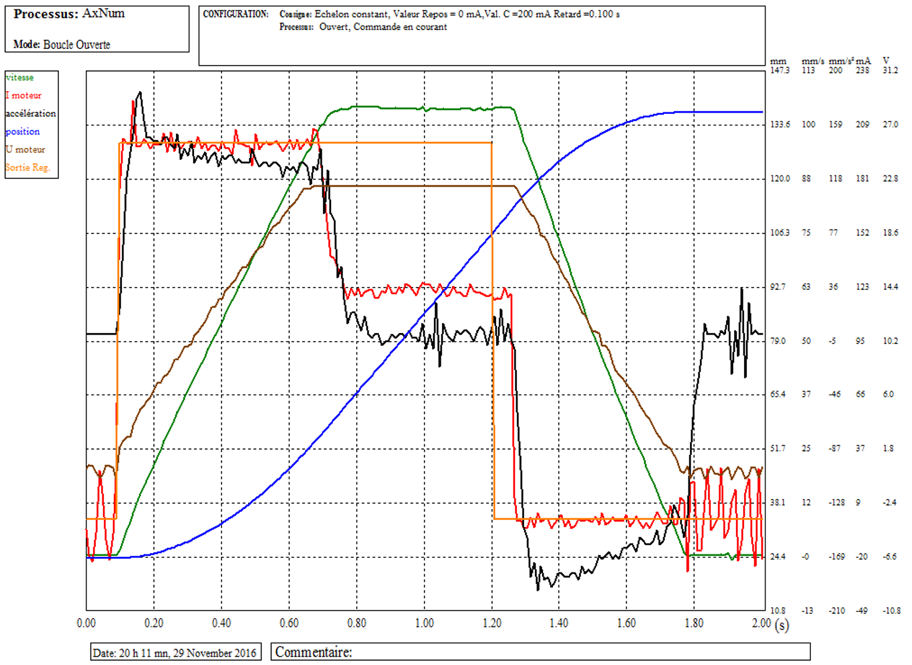
\includegraphics[width=1.0\textwidth]{images/figure3.png}
\caption{Résultats expérimentaux boucle ouverte \label{figure3}}
\end{center}
\end{figure}


\FloatBarrier
\subsubsection{Amélioration du modèle en boucle ouverte}

Le modèle accélère trop fort car les frottements sont négligés. On constate que 50mA sont nécessaire pour mettre l'Axnum en mouvement (effet de frottement sec). 

\question{Placer un bloc « Discontinuities/Deadzone » avant le moteur pour prendre en compte cet effet. Exécuter de nouveau la comparaison et observer l'amélioration.}

\question{Dans un second temps on peut ajouter des frottements visqueux. Pour cela une force proportionnelle à la vitesse  est ajoutée lors du bilan des forces. Il faut ajouter un additioneur (block « add ») pour faire le nouveau bilan des forces (avant le calcul de l'accélération). A l'aide d'un gain et d'un sommateur (commonly used block) mettre en place le frottement visqueux ($f=1$).}

\question{Au bout de $0,7s$ le système s'arrête brutalement d'accélérer (vitesse constante) contrairement au modèle. En observant la mesure de tension proposer une explication à cette limitation. On pourra aussi raisonner sur le comportement sur un temps long du modèle comparé à la mesure et sa pertinence.}

On doit obtenir la figure ci-dessous.

\begin{center}
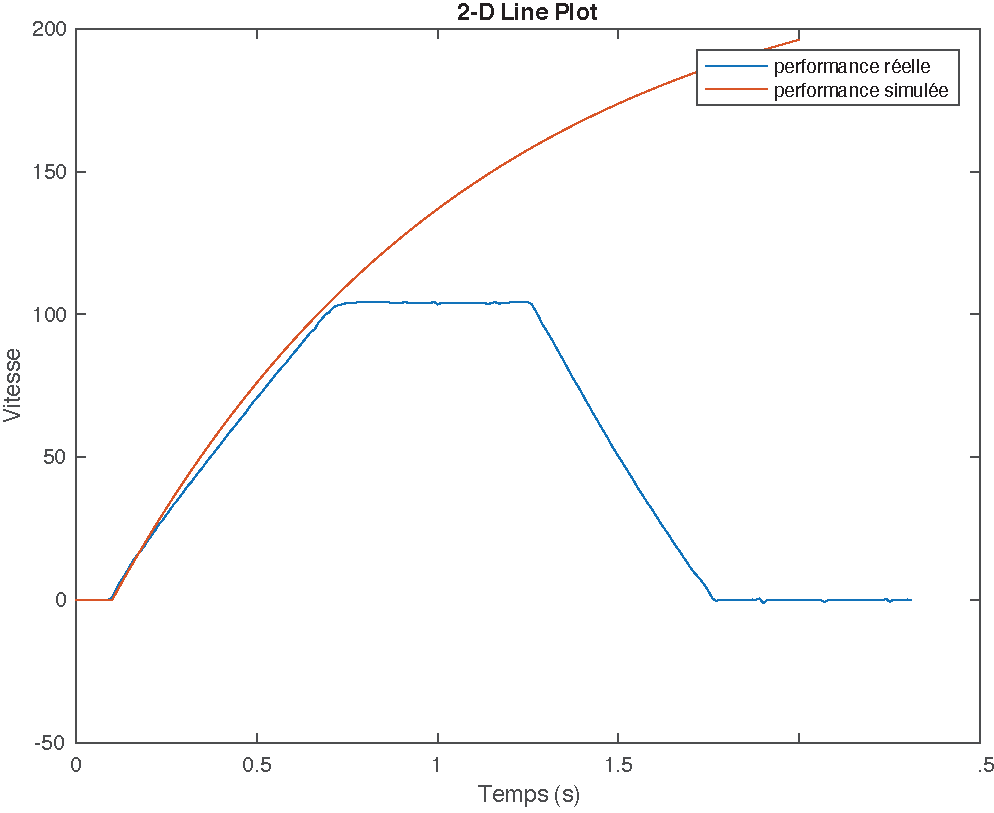
\includegraphics[width=0.7\textwidth]{images/figure_bo.pdf}
\end{center}

\subsection{Recherche des performances en boucle fermé du système}
\subsubsection{Modélisation en boucle fermée : construction du schéma bloc.}

Le capteur de vitesse on le considèrera idéal et un retour unitaire de la vitesse sera utilisé. Une conversion m/s mm/s restera nécessaire avant le comparateur.


\question{En vous appuyant du schéma ci-dessous donné par le logiciel, identifier l'entrée et la sortie du modèle puis construire le schéma bloc en boucle fermé du système.}

\begin{center}
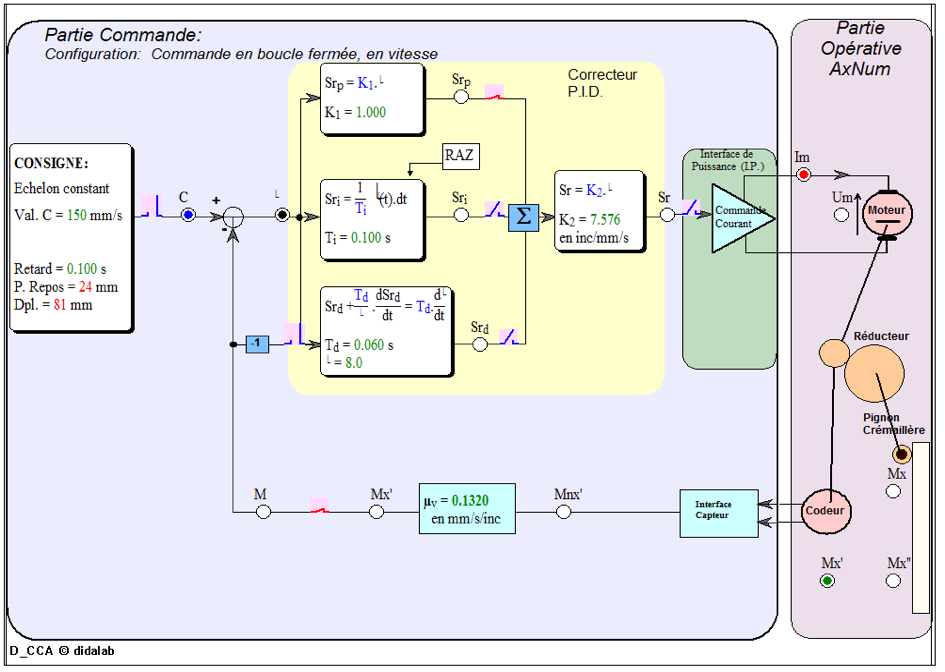
\includegraphics[width=1.0\textwidth]{images/BF_logiciel.png}
\end{center}


\question{Prévoir d'exporter les données dans le workspace sous le nom "mxp$\_$bf".}

\question{Modifier le nom de la variable dans le bloc workspace ("mxp$\_$bf2") et réaliser une simulation avec un gain proportionnel égal à 2.}

\subsubsection{Comparaison des performances.}

\question{Exécuter le script compareBF pour afficher la courbe de simulation et la courbe expérimentale (Figure \ref{figure3}). Les résultats expérimentaux sont aussi disponibles dans la figure « BFV100VIK1.csv ». Commenter les écarts.}

On dispose du fichier de données expérimentales obtenues avec un gain du correcteur proportionnel égal à $2$.

\question{Modifier le programme pour comparer les résultats (fichier de données expérimental : BFV100VIK2.csv).}

On doit obtenir la figure ci-dessous.

\begin{center}
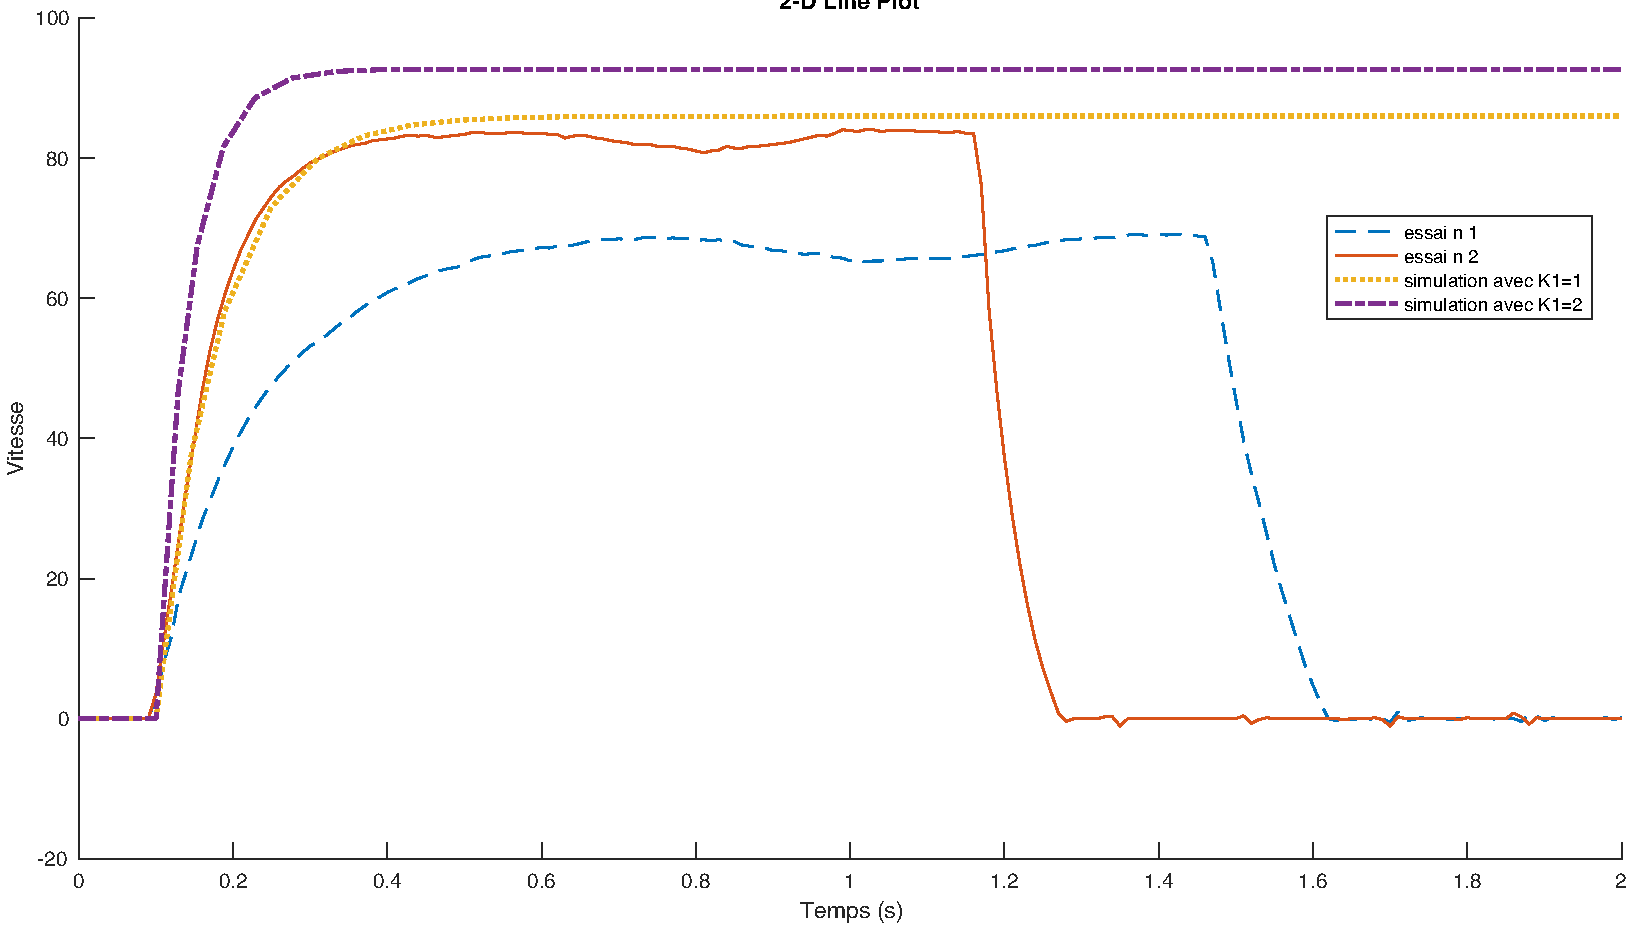
\includegraphics[width=0.7\textwidth]{images/figure_bf.pdf}
\end{center}

\question{Modifier la valeur de $f$ pour réduire au mieux les écarts entre performances réelles et simulées.}

\subsection{Simulation en boucle fermée de position, interface de courant}

\question{A l'aide de la figure ci-dessous réaliser le schéma bloc de la simulation en boucle fermée de position avec interface de courant.}

\begin{center}
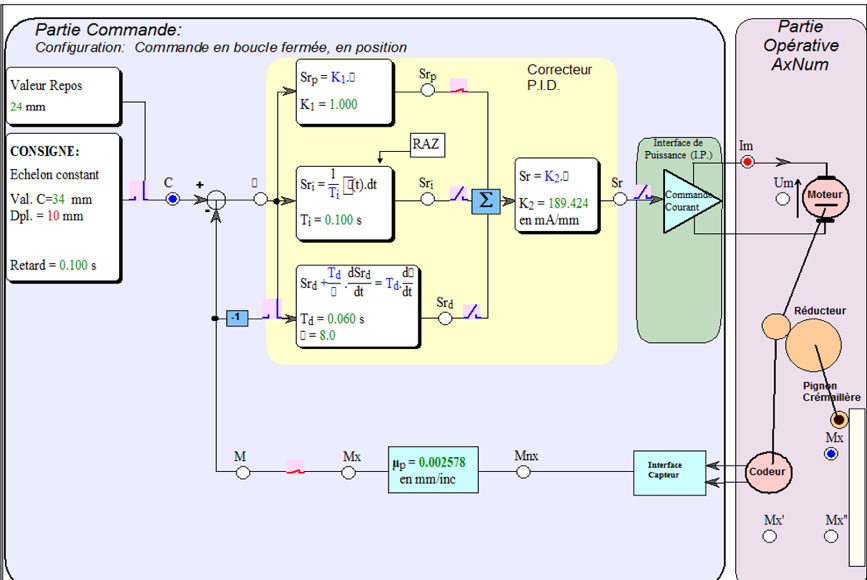
\includegraphics[width=1.0\textwidth]{images/logiciel_BF_position.png}
\end{center}


\subsection{Annexe}
\subsubsection{documentation du motoréducteur/pignon SMH}
\begin{figure}[!htb]
\begin{center}
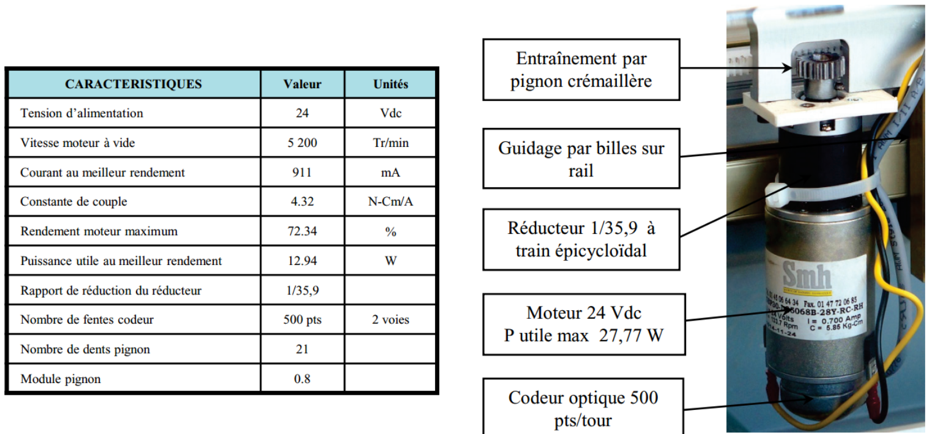
\includegraphics[width=1.0\textwidth]{images/moteur.png}
\end{center}
\end{figure}
\FloatBarrier
\subsubsection{Utilisation du logiciel de commande de l'axe numérique}
\begin{itemize}
\item Il faut lancer le logiciel (icône sur le bureau).
\item Il est possible qu'on demande de configurer le port de communication. Il faut alors choisir le bon port com (généralement com3 ou vérifier dans le gestionnaire de périphérique) puis relancer le logiciel.
\item Dans le menu \textbf{Choisir} : 
\begin{itemize}
\item mode de commande : \textbf{boucle ouverte}
\item Interface de de commande : \textbf{Commande courant}
\begin{center}
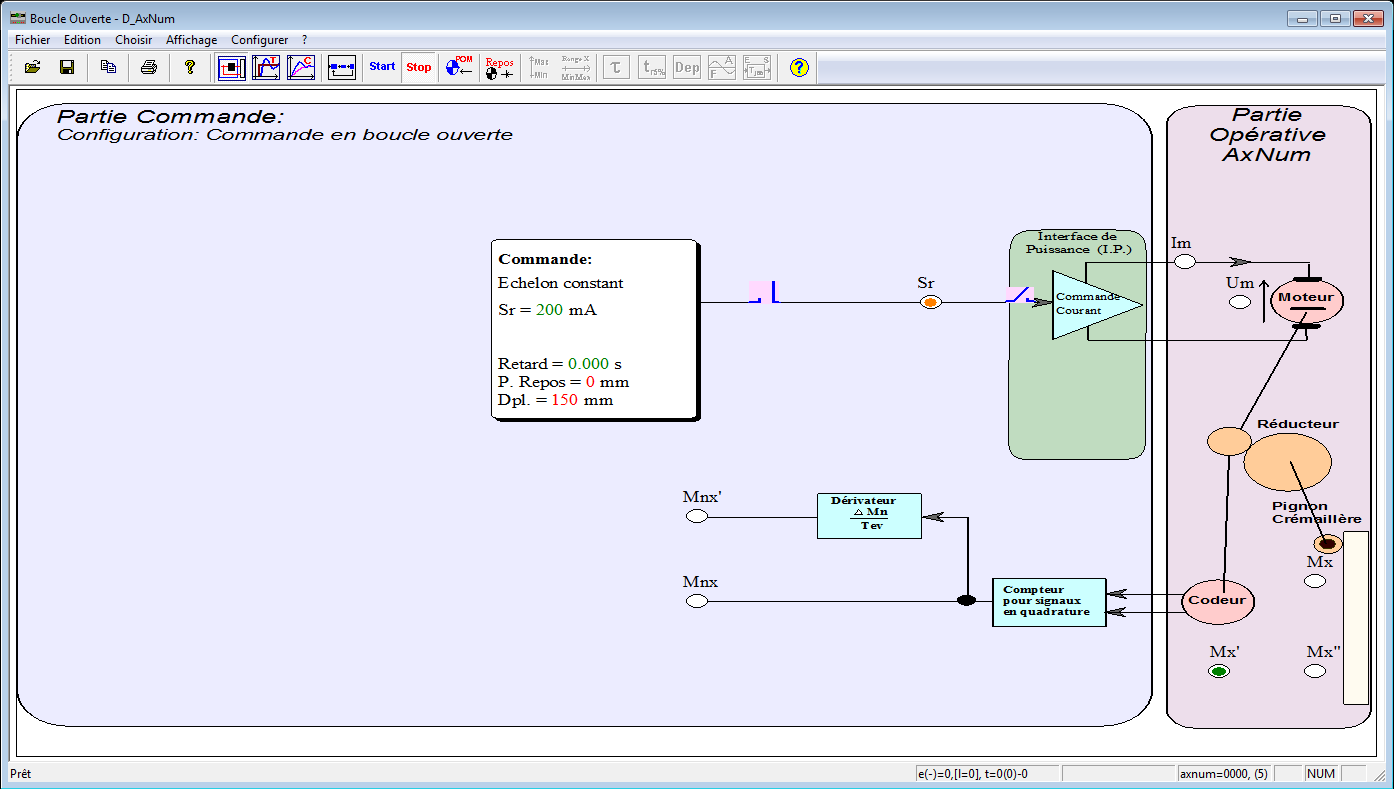
\includegraphics[width=0.9\textwidth]{images/logiciel2.png}
\end{center} 
\item unité : sortie régulateur : \textbf{unité IP}
\begin{center}
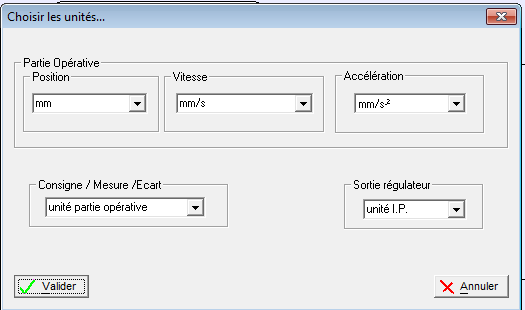
\includegraphics[width=0.6\textwidth]{images/logiciel_unite.png}
\end{center}
\item Dans le menu \textbf{Configurer : } Valeurs initiales
\item Dans la case \textbf{Commande} choisir une entrée de type échelon d'amplitude $200mA$ en BO et $100mm/s$ en BF.
\item Choisir les signaux et cocher si possible dans l'ordre : 
\begin{itemize}
\item En \textbf{BO} : Consigne, Ecart, I moteur, vitesse ; 
\item en \textbf{BF} : Vitesse, Imot, accéération, position, Umot, sortie Reg.
\end{itemize}
\item Pour lancer l'essai : 
\begin{enumerate}
\item Fermer l'interrupteur de l'interface de puissance ; 
\item Fermer l'interrupteur directement en aval de la commande ; 
\item Visualiser les résultats en cliquant sur 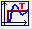
\includegraphics[width=0.1\textwidth]{images/icone.png}
\end{enumerate}
\end{itemize}

\end{itemize}